\chapter{Detailed Video Evaluation Methodology}
\label{app:video_evaluation_details}

This appendix provides additional details and supporting results for the video processing evaluation in Section~\ref{sec:video_processing_results}. Section~\ref{sec:video_processing_results} reports the main system-level results, while this appendix documents the test material, evaluation setup, annotation procedure, metrics, temporal coverage test, and additional failure-case analysis.

\section{Evaluation Setup}

The video evaluation was performed as a system-level extension of the image detection and redaction pipeline. The tests focused on detection frequency, automatic prediction, and manual tracking. They were performed on three short videos with different resolutions, orientations, and durations. Each video was processed using different values of \texttt{detect\_every}, where lower values run detection more frequently and higher values rely more on prediction between detection frames.

\begin{table}[H]
\centering
\begin{tabular}{lcccc}
\toprule
\textbf{Video} & \textbf{Resolution} & \textbf{Frames} & \textbf{Duration} & \textbf{\acrshort{fps}} \\
\midrule
car\_video & $1280\times720$ & 153 & 5.10 s & 30.00 \\
walk & $854\times480$ & 360 & 12.00 s & 30.00 \\
face\_track & $720\times1280$ & 270 & 9.14 s & 29.55 \\
\bottomrule
\end{tabular}
\caption{Overview of videos used for evaluating the video processing pipeline.}
\label{tab:video_test_material}
\end{table}

The evaluation focused on three main aspects. First, automatic Kalman-based prediction was evaluated to determine whether propagated \gls{bounding box}es remained accurate between detection frames. Second, manual tracking was evaluated to determine whether a user-selected object could be followed across a video sequence. Third, processing performance was measured to evaluate how different detection intervals affected runtime.

\section{Ground-Truth Annotation}

Automatic prediction was evaluated by comparing the generated frame-wise manifests with human-labeled ground-truth boxes. The \texttt{detect\_every = 1} configuration was used as a full-detection baseline, but it was excluded from the Kalman prediction accuracy results because no intermediate non-detection frames exist in this configuration. Since every frame receives detector output, the Kalman filter does not need to estimate object positions between detection frames in this case.

For the remaining configurations, predicted boxes were compared with human-labeled boxes on non-detection frames. These frames are important because they represent cases where the system relies on Kalman prediction instead of new detector output.

For manual tracking, the car was first manually annotated on sampled frames across the \texttt{car\_video} video. The manual tracker was then initialized from a ground-truth box in the middle of the video, and the predicted boxes were compared with the human-labeled boxes using \acrshort{iou}.

\section{Evaluation Metrics}

The evaluation used \acrshort{iou} and sensitive-region coverage as the main accuracy metrics.

\paragraph{Intersection over Union}

\acrshort{iou} measures how closely the predicted box aligns with the human-labeled box. It is calculated as the overlap between the predicted and ground-truth boxes divided by their union.

\[
IoU = \frac{Area(B_p \cap B_g)}{Area(B_p \cup B_g)}
\]

where \(B_p\) represents the predicted box and \(B_g\) represents the ground-truth box.

\paragraph{Sensitive-Region Coverage}

Sensitive-region coverage measures how much of the human-labeled sensitive region was covered by the predicted box. This metric was included because anonymization does not only depend on tight localization. A box can be slightly less precise but still cover the sensitive content sufficiently for redaction.

\section{Temporal Coverage Test}

Before evaluating prediction accuracy against human-labeled ground truth, a temporal coverage test was performed. The purpose of this test was not to measure exact tracking accuracy, but to measure whether Kalman-based prediction preserved active \gls{bounding box}es across frames where full detection was not executed.

Since full detection is only executed on selected frames, a detection-only manifest would only contain detected boxes on those frames. Automatic Kalman-based prediction was therefore compared with this detection-frame-only estimate to evaluate whether it preserved the \gls{bounding box}es across non-detection frames.

\begin{table}[H]
\centering
\begin{tabular}{rccc}
\toprule
\textbf{\texttt{detect\_every}} & \textbf{Detection calls} & \textbf{Detection-only} & \textbf{Manifest with prediction} \\
\midrule
1  & 261.00 & 99.44\% & 99.44\% \\
2  & 130.67 & 50.02\% & 99.63\% \\
5  & 52.33  & 20.09\% & 99.63\% \\
10 & 26.33  & 10.15\% & 99.17\% \\
\bottomrule
\end{tabular}
\caption{Average frame coverage across the three tested videos. ``Detection-only'' estimates the percentage of frames that would contain boxes if boxes were only used on frames where full detection was executed. ``Manifest with prediction'' shows the percentage of frames with active boxes after Kalman-based prediction has propagated boxes between detection frames.}
\label{tab:video_temporal_coverage}
\end{table}

Kalman-based prediction substantially increased bounding-box coverage when detection was run less frequently. With \texttt{detect\_every = 10}, the detection-frame estimate was 10.15\%, while the prediction-based manifest maintained 99.17\% coverage on average. This confirms that the prediction step filled the gaps between detection frames and produced continuous boxes for later review and redaction.

However, this metric should be interpreted only as a temporal coverage result. It shows whether boxes were present in the frame-wise manifest, but it does not show whether the boxes were accurately aligned with the sensitive objects. For this reason, the main video evaluation in Section~\ref{sec:video_processing_results} uses human-labeled ground truth, \acrshort{iou}, and sensitive-region coverage as the primary accuracy results.

\section{Processing-Time Benchmark Setup}

Processing performance was evaluated using the same \texttt{detect\_every} values as the prediction accuracy evaluation. Each configuration was run three times after a warmup run, and the reported values were averaged across the three tested videos. The benchmark was executed on CPU.

The measured processing time included the complete video processing path used in the evaluation, including frame decoding, selected frame-level detection calls, prediction between detection frames, and manifest generation. The purpose of the benchmark was to measure how reducing the number of detection calls affected total processing cost.

\section{Worst-Frame Example}

Figure~\ref{fig:video_prediction_worst_frame} shows the lowest-quality frame found in the \texttt{car\_video} sequence when using \texttt{detect\_every = 10}. This example was selected from the human-labeled evaluation and illustrates a difficult case with several nearby moving vehicles.

\begin{figure}[H]
\centering
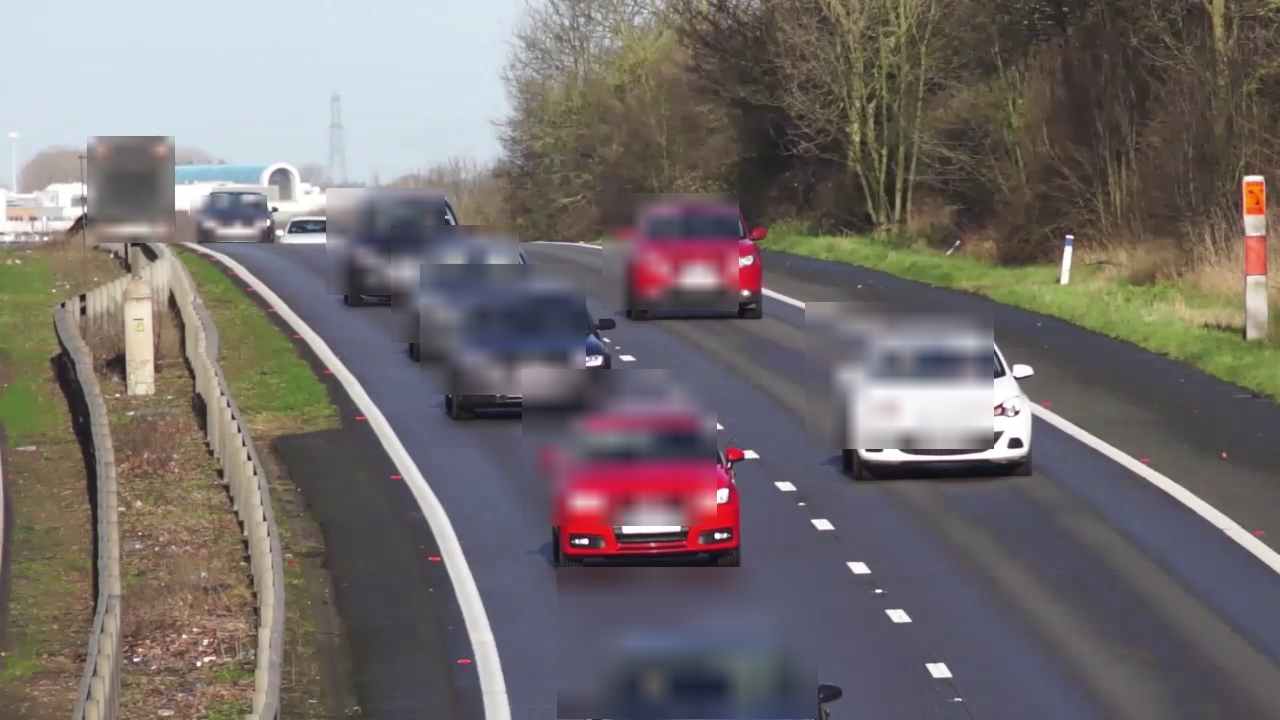
\includegraphics[width=0.85\textwidth]{figures/images/chapter-11/car_kalman_worst_frame.png}
\caption{Worst-frame example from the \texttt{car\_video} sequence using \texttt{detect\_every = 10}. The frame contained nine human-labeled vehicle boxes and ten predicted boxes. The mean \acrshort{iou} was 0.5245, while mean sensitive-region coverage was 0.7469. This illustrates that long prediction intervals can reduce localization accuracy in frames with several nearby moving objects.}
\label{fig:video_prediction_worst_frame}
\end{figure}

This example shows why both \acrshort{iou} and sensitive-region coverage were used in the main evaluation. The predicted boxes still cover large parts of the sensitive regions, but the alignment is less precise than in easier frames. This makes the frame useful as a qualitative example of the limitations of longer prediction intervals.

The lower \acrshort{iou} in this frame was mainly caused by several nearby moving vehicles that produced overlapping prediction paths between sparse detection frames. This type of scenario is more challenging for prediction than isolated objects with stable movement. The example supports the main result that \texttt{detect\_every = 10} provides the largest runtime reduction, but also increases the risk of localization drift in crowded or fast-moving scenes.